% Copyright 2009--2024  Ed Bueler

\documentclass[10pt,hyperref]{beamer}

\mode<presentation>
{
  \usetheme{Madrid}

  \usecolortheme{beaver}

  \setbeamercovered{transparent}
  
  \setbeamerfont{frametitle}{size=\large}
}

\usepackage[english]{babel}
\usepackage[latin1]{inputenc}
\usepackage{times}
\usepackage[T1]{fontenc}
% Or whatever. Note that the encoding and the font should match. If T1
% does not look nice, try deleting the line with the fontenc.

\usepackage{empheq}
\usepackage{animate}
\usepackage{xspace}
\usepackage{fancyvrb}
\usepackage{hyperref}



\title{\emph{How} to put a polynomial through points}

\author{Ed Bueler}

\institute{MATH 426 Numerical Analysis}

\date{September 2024}
\date{}



% If you wish to uncover everything in a step-wise fashion, uncomment
% the following command: 
%\beamerdefaultoverlayspecification{<+->}

\newcommand{\bb}{\mathbf{b}}
\newcommand{\bx}{\mathbf{x}}
\newcommand{\bv}{\mathbf{v}}
\newcommand{\bw}{\mathbf{w}}

\newcommand{\ddt}[1]{\ensuremath{\frac{\partial #1}{\partial t}}}
\newcommand{\ddx}[1]{\ensuremath{\frac{\partial #1}{\partial x}}}
\renewcommand{\t}[1]{\texttt{#1}}
\newcommand{\Matlab}{\textsc{Matlab}\xspace}
\newcommand{\Octave}{\textsc{Octave}\xspace}
%\newcommand{\MO}{\Matlab/\Octave}
\newcommand{\MO}{\Matlab}
\newcommand{\eps}{\epsilon}

\newcommand{\MS}{\alert{MAKE SURE}\xspace}

\newcommand{\exer}[2]{\medskip\noindent \textbf{#1.}\quad #2}

\newcommand{\mfile}[1]{
\VerbatimInput[frame=single,label=\fbox{\scriptsize \textsl{\,#1\,}},fontfamily=courier,fontsize=\scriptsize]{#1}
}

\newcommand{\mfiletiny}[1]{
\VerbatimInput[frame=single,label=\fbox{\scriptsize \textsl{\,#1\,}},fontfamily=courier,fontsize=\tiny]{#1}
}


\AtBeginSection[]
{
  \begin{frame}<beamer>
    \frametitle{Outline}
    \tableofcontents[currentsection,hideallsubsections]
  \end{frame}
}

\begin{document}

\begin{frame}
  \maketitle
\end{frame}


\begin{frame}{purpose}
\begin{quote}
The topic of these slides is covered in Chapter 8 of the text.\footnote{Greenbaum \& Chartier, \emph{Numerical Methods: Design, Analysis, and Computer Implementation of Algorithms}, Princeton University Press 2012).}  When we get there we will be more thorough.

\bigskip
The emphasis here, in these slides, is on \alert{how} to put a polynomial through points.  The polynomial interpolation error theorem (Chapter 8), addresses the ``how good is the result'' question.  While it is a good idea to look at Chapter 8, it is not needed for understanding these slides or for doing Assignment \#3.
\end{quote}
\end{frame}

\begin{frame}{an example of the problem}

\begin{itemize}
\item suppose you have a function $y=f(x)$ which goes through these points:
   $$(-1,2), \quad (0,3), \quad (3,4), \quad (5,0)$$
\item the $x$-coordinates of these points are not equally-spaced!
  \begin{itemize}
  \item[$\circ$]  in these notes I will \emph{never} assume the $x$-coordinates are equally-spaced
  \end{itemize}
\item name the points $(x_i,y_i)$, for $i=1,2,3,4$
\item there is a polynomial $P(x)$ of degree 3 which goes through these points
\item we will build it concretely
\item we will show later that there is only one such polynomial
\end{itemize}
\end{frame}


\begin{frame}{a picture of the problem}

\begin{itemize}
\item figure below shows the points from the previous slide
\item they may be values of a function $f(x)$ \dots but we don't know or see that function

\medskip
  \begin{center}
  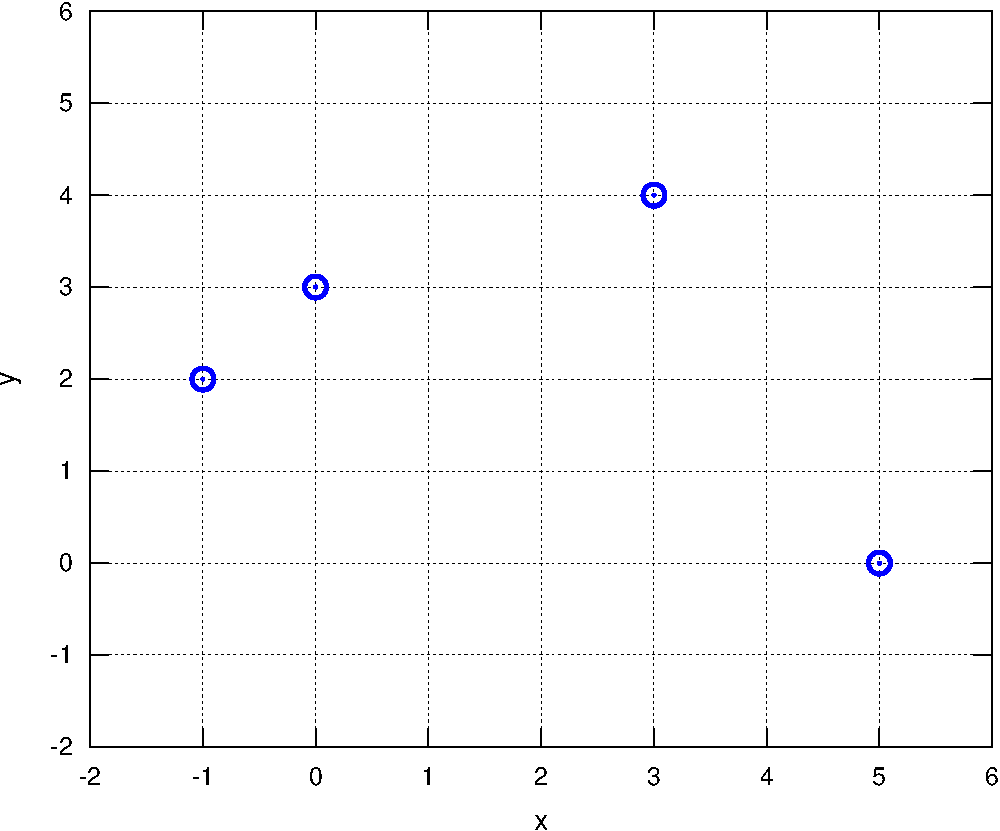
\includegraphics[width=0.6\textwidth]{ex1}
  \end{center}
\end{itemize}
\end{frame}


\begin{frame}{how to find $P(x)$}

\begin{itemize}
\item suppose $P(x)$ is the degree 3 polynomial through the 4 points
\item a standard way to write it is:
	$$P(x) = c_0 + c_1 x + c_2 x^2 + c_3 x^3$$
\item \emph{note}: there are 4 unknown coefficients and 4 points
  \begin{itemize}
  \item[$\circ$] degree $n-1$ polynomials have the right length for $n$ points
  \end{itemize}
\item the facts ``$P(x_i)=y_i$'' for the given points gives 4 linear equations in 4 unknowns:
\begin{align*}
c_0 + c_1 (-1) + c_2 (-1)^2 + c_3 (-1)^3 &= 2 \\
c_0 + c_1 (0) + c_2 (0)^2 + c_3 (0)^3 &= 3 \\
c_0 + c_1 (3) + c_2 (3)^2 + c_3 (3)^3 &= 4 \\
c_0 + c_1 (5) + c_2 (5)^2 + c_3 (5)^3 &= 0
\end{align*}
\item \MS that you are clear on how I got these equations, and that you can do the same thing in an example with different points or different polynomial degree
\end{itemize}
\end{frame}


\begin{frame}{a linear system}
\begin{itemize}
\item you can solve the equations by hand \dots that would be tedious
\item you are allowed a wand \dots I mean a \MO
\item the system has a matrix form ``$A\, \bv = \bb$'' with $\bv$ unknown:
$$\begin{bmatrix}
1 & -1 & (-1)^2 & (-1)^3 \\
1 & 0 & 0^2 & 0^3 \\
1 & 3 & 3^2 & 3^3 \\
1 & 5 & 5^2 & 5^3
\end{bmatrix}\begin{bmatrix}
c_0 \\ c_1 \\ c_2 \\ c_3
\end{bmatrix}
=
\begin{bmatrix}
2 \\ 3 \\ 4 \\ 0
\end{bmatrix}$$
\item I am not simplifying the numbers in the matrix \dots because:
  \begin{itemize}
  \item[$\circ$] a machine can do that, and 
  \item[$\circ$] the pattern is what matters\footnote{often you should keep things unsimplified if they are going to become code}
  \end{itemize}
\item \MS you can convert from the original ``fit a polynomial through these points'' question into the matrix form ``$A\, \bv = \bb$''
\end{itemize}
\end{frame}


\begin{frame}[fragile]
\frametitle{how to \emph{easily} find $P(x)$}
  
\begin{itemize}
\item \MO is designed to solve linear systems \dots easily!
\item enter the matrix and the known vector into \MO:

\begin{Verbatim}[frame=single,fontfamily=courier,fontsize=\scriptsize]
>> A = [1 -1 (-1)^2 (-1)^3; 1 0 0^2 0^3; 1 3 3^2 3^3; 1 5 5^2 5^3]
A =
     1    -1     1    -1
     1     0     0     0
     1     3     9    27
     1     5    25   125
>> b = [2; 3; 4; 0]
b =
   2
   3
   4
   0
\end{Verbatim}
\item solve the linear system to get $\bv=[c_0\, c_1\, c_2\, c_3]$:
\begin{Verbatim}[frame=single,fontfamily=courier,fontsize=\scriptsize]
>> v = A \ b
v =
   3.000000
   0.983333
  -0.066667
  -0.050000
\end{Verbatim}
\item so the polynomial is $P(x) = 3 + 0.983333 x - 0.066667 x^2 - 0.05 x^3$
\end{itemize}
\end{frame}


\begin{frame}[fragile]
\frametitle{did we solve the problem?}

\begin{itemize}
\item the polynomial we found does go through the points:

\medskip
\begin{Verbatim}[frame=single,fontfamily=courier,fontsize=\scriptsize]
>> 3.000000 + 0.983333*(-1) - 0.066667*(-1)^2 -0.050000*(-1)^3
ans =  2
>> 3.000000 + 0.983333*(0) - 0.066667*(0)^2 -0.050000*(0)^3
ans =  3
>> 3.000000 + 0.983333*(3) - 0.066667*(3)^2 -0.050000*(3)^3
ans =  4.0000
>> 3.000000 + 0.983333*(5) - 0.066667*(5)^2 -0.050000*(5)^3
ans = -1.0000e-05
\end{Verbatim}

\medskip
  \begin{center}
  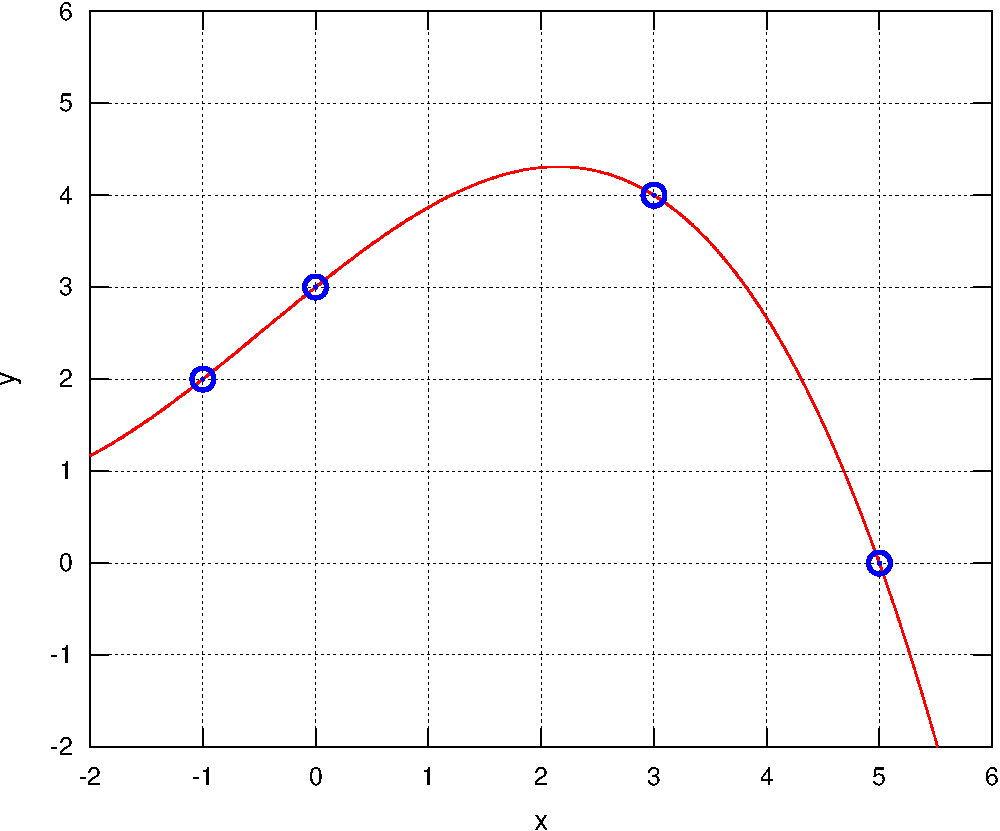
\includegraphics[width=0.45\textwidth]{ex1solved}
  \end{center}
\end{itemize}
\end{frame}


\begin{frame}[fragile]
\frametitle{summary: linear systems in \MO}

\begin{itemize}
\item before we move on, here is a summary of some basics
\item you enter matrices like $A$ by rows
  \begin{itemize}
  \item[$\circ$] spaces separate entries
  \item[$\circ$] semicolons separate rows
  \end{itemize}
\item column vectors like $\bb$ are just matrices with one column
  \begin{itemize}
  \item[$\circ$] to quickly enter column vectors use the transpose operation:
  \end{itemize}
\begin{Verbatim}[frame=single,fontfamily=courier,fontsize=\scriptsize]
>> b = [2 3 4 0]'
b =
   2
   3
   4
   0
\end{Verbatim}
\item to solve the system $A\, \bv = \bb$ we ``divide by'' the matrix: $\bv = A^{-1} \bb$ \dots but this is \emph{left} division; \MO has a single-character \emph{backslash} operation:
\begin{Verbatim}[frame=single,fontfamily=courier,fontsize=\scriptsize]
>> v = A \ b
\end{Verbatim}

\bigskip
\scriptsize
\item the forward slash does not work because of the sizes of the matrix and the vector are not right:
\begin{Verbatim}[frame=single,fontfamily=courier,fontsize=\scriptsize]
>> v = b / A  % NOT CORRECT for our A and b; wrong sizes
\end{Verbatim}
\end{itemize}
\end{frame}


\begin{frame}{the general case}

\begin{itemize}
\item suppose we have $n$ points $(x_i,y_i)$ with distinct $x$-coordinates
  \begin{itemize}
  \item[$\circ$]  for example, if $n=4$ we have points $(x_1,y_1),\,(x_2,y_2),\,(x_3,y_3),\,(x_4,y_4)$
  \end{itemize}
\item then the polynomial has degree one less:  the polynomial $P(x)$ which goes through the $n$ points has degree $n-1$
\item the polynomial has this form:
	$$P(x) = c_0 + c_1 x + c_2 x^2 + \dots + c_{n-1} x^{n-1}$$
\item the equations which determine $P(x)$ say that \emph{the polynomial goes through the points}:
	$$P(x_i) = y_i \qquad \text{for} \quad i=1,2,\dots,n$$
\item this is a system of $n$ equations of this form:
	$$c_0 + c_1 x_i + c_2 x_i^2 + \dots + c_{n-1} x_i^{n-1} = y_i \qquad \text{for} \quad i=1,2,\dots,n$$
\item the $n$ coefficients $c_i$ are unknown, while the $x_i$ and $y_i$ are known
\end{itemize}
\end{frame}


\begin{frame}[fragile]
\frametitle{the pattern in the matrix}

\begin{itemize}
\item as a matrix:
	$$A = \begin{bmatrix}
	1 & x_1 & x_1^2 & \dots & x_1^{n-1} \\
	1 & x_2 & x_2^2 & \dots & x_2^{n-1} \\
	 & \vdots & & \ddots &  \\
	1 & x_n & x_n^2 & \dots & x_n^{n-1} \\
	\end{bmatrix}$$
\item and $\bb$ is a column vector with entries $y_i$:\quad  $\bb = [y_1\quad y_2 \quad \dots \, y_n]'$
\item as before, this gives a system of $n$ equations:\quad $A\, \bv = \bb$
\item the matrix $A$ is called a \emph{Vandermonde matrix}\footnote{Alexandre-Th\'eophile Vandermonde, in papers on determinants in 1772}
\end{itemize}
\end{frame}


\begin{frame}[fragile]
\frametitle{the Vandermonde matrix is a built-in}

\begin{itemize}
\item actually, Vandermonde matrices are already built-in to \MO
\item for example, the Vandermonde matrix $A$ for our original four points $(-1,2), (0,3), (3,4), (5,0)$ is

\begin{Verbatim}[frame=single,fontfamily=courier,fontsize=\scriptsize]
>> vander([-1 0 3 5])
ans =
    -1     1    -1     1
     0     0     0     1
    27     9     3     1
   125    25     5     1
\end{Verbatim}
\item two comments:
  \begin{itemize}
  \item[$\circ$] oops!  the columns are in reversed order, compared to our choice
  \item[$\circ$] note that \emph{only} the $x$-coordinates are needed to build $A$, and not the $y$-coordinates
  \end{itemize}
\item fix the column order to agree with our earlier choice using ``\texttt{fliplr}'' (flip left-to-right):
\begin{Verbatim}[frame=single,fontfamily=courier,fontsize=\scriptsize]
>> A = fliplr(vander([-1 0 3 5]))
A =
     1    -1     1    -1
     1     0     0     0
     1     3     9    27
     1     5    25   125
\end{Verbatim}
\end{itemize}
\end{frame}


\begin{frame}[fragile]
\frametitle{example of the Vandermonde matrix method}

\begin{itemize}
\item a complete code to solve our 4-point problem:

\bigskip
\begin{Verbatim}[frame=single,fontfamily=courier,fontsize=\scriptsize]
  A = fliplr(vander([-1 0 3 5]));
  b = [2 3 4 0]';
  v = A \ b
\end{Verbatim}
\bigskip

\item after the coefficents\, \texttt{v}\, are computed, they form $P(x)$ this way:
	$$P(x) = \text{\texttt{v(1)}} + \text{\texttt{v(2)}}\, x + \text{\texttt{v(3)}}\, x^2 + \dots + \text{\texttt{v(n)}}\, x^{n-1}$$

\item thus we can plot the 4 points and the polynomial this way:
\bigskip
\begin{Verbatim}[frame=single,fontfamily=courier,fontsize=\scriptsize]
  plot([-1 0 3 5],[2 3 4 0],'o','markersize',12)
  x = -2:0.01:6;
  P = v(1) + v(2)*x + v(3)*x.^2 + v(4)*x.^3;
  hold on,  plot(x,P,'r'),  hold off,  xlabel x,  ylabel y
\end{Verbatim}
\bigskip

\item this was the graph shown a few slides back
\end{itemize}
\end{frame}


\begin{frame}[fragile]
\frametitle{example of \texttt{polyfit}}

\begin{itemize}
\item actually we don't even need to call \texttt{vander} ourselves, because polynomial interpolation is built-in to \MO:

\bigskip
\begin{Verbatim}[frame=single,fontfamily=courier,fontsize=\scriptsize]
  v = polyfit([-1 0 3 5], [2 3 4 0], 3)
\end{Verbatim}
\bigskip

\item the only difference is that the coefficient order is reversed:
	$$P(x) = \text{\texttt{v(n)}} + \text{\texttt{v(n-1)}}\, x + \dots + \text{\texttt{v(1)}}\, x^{n-1}$$

\item plot using the ``evaluate a polynomial'' built-in called \texttt{polyval()}:

\bigskip
\begin{Verbatim}[frame=single,fontfamily=courier,fontsize=\scriptsize]
  plot([-1 0 3 5],[2 3 4 0],'o','markersize',12)
  x = -2:0.01:6;
  P = polyval(v,x);
  hold on,  plot(x,P,'r'),  hold off,  xlabel x,  ylabel y
\end{Verbatim}
\bigskip
\end{itemize}
\end{frame}


\begin{frame}{Lagrange's idea (1795): no systems at all!}

\begin{itemize}
\item a new idea, illustrated with the same points\quad  $(-1,2), (0,3), (3,4), (5,0)$
\item Lagrange (and others) could directly write down four polynomials corresponding to the $x$-coordinates $x_1,\dots,x_4$:
\small
\begin{align*}
\ell_{1}(x) &= \frac{(x-x_2)(x-x_3)(x-x_4)}{(x_1-x_2)(x_1-x_3)(x_1-x_4)} = \frac{x (x-3) (x-5)}{(-1)(-4)(-6)} \\
\ell_{2}(x) &= \frac{(x-x_1)(x-x_3)(x-x_4)}{(x_2-x_1)(x_2-x_3)(x_2-x_4)} = \frac{(x+1) (x-3) (x-5)}{(1)(-3)(-5)} \\
\ell_{3}(x) &= \frac{(x-x_1)(x-x_2)(x-x_4)}{(x_3-x_1)(x_3-x_2)(x_3-x_4)} = \frac{(x+1) (x) (x-5)}{(4)(3)(-2)} \\
\ell_{4}(x) &= \frac{(x-x_1)(x-x_2)(x-x_3)}{(x_4-x_1)(x_4-x_2)(x_4-x_3)} = \frac{(x+1) (x) (x-3)}{(6)(5)(2)}
\end{align*}
\normalsize
\item these are called the \emph{Lagrange polynomials}
\item the \emph{pattern}:
  %\renewcommand{\labelenumi}{}
  \begin{enumerate}
  \item numerator and denominator have similar structure
  \item \dots but the denominators are constant
  \item $\ell_i(x)$ has no ``$(x-x_i)$'' factor in the numerator
  \item $\ell_i(x)$ has no ``$(x_i-x_i)$'' factor in the denominator
  \item as long as the $\{x_i\}$ are distinct, we never divide by zero
  \end{enumerate}
\end{itemize}
\end{frame}


\begin{frame}{Lagrange's idea: polynomials which ``hit one point''}

\begin{itemize}
\item consider a plot of $\ell_1(x)$, $\ell_2(x)$, $\ell_3(x)$, $\ell_4(x)$:
  \begin{center}
  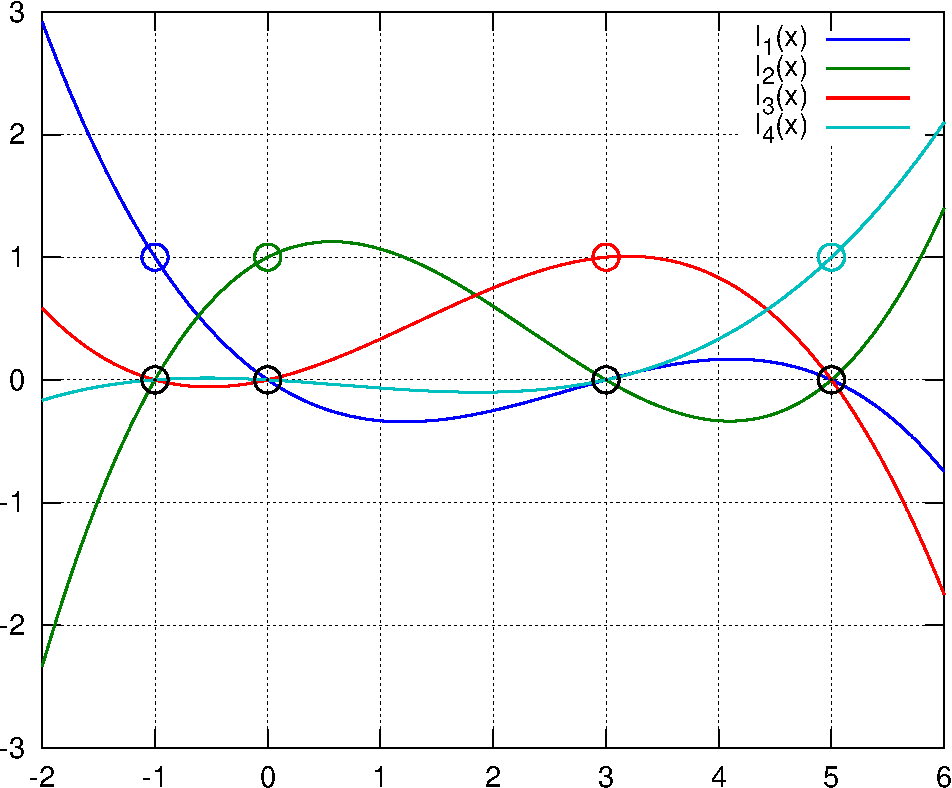
\includegraphics[width=0.4\textwidth]{lagrange4}
  \end{center}
\item a crucial pattern emerges:
\begin{quote}
the polynomial $\ell_i(x)$ has value 0 at all of the $x$-values of the points, except that it is 1 at $x_i$
\end{quote}
\item \MS make sure you can find the Lagrange polynomials if I give you the $x$-values of $n$ points
\item but why is this helpful?
\end{itemize}
\end{frame}


\begin{frame}{Lagrange's idea, cont.}

\begin{itemize}
\item the picture on the last page illustrates what is generally true of the Lagrange polynomials:
	$$\ell_i(x_j) = \begin{cases}
   	                 1, & j = i, \\
   	                 0, & \text{otherwise}.
	                \end{cases}$$
\item so why does this help find $P(x)$?
\item recall that we have values $y_i$ which we want the polynomial $P(x)$ to ``hit''
\item that is, we \emph{want} this to be true for each $i$:
	$$P(x_i) = y_i$$
\item \emph{thus the answer is}:
	$$P(x) = y_1 \ell_1(x) + y_2 \ell_2(x) + y_3 \ell_3(x) + y_4 \ell_4(x)$$
\end{itemize}
\end{frame}


\begin{frame}{Lagrange's idea, $\text{cont.}^2$}

\begin{itemize}
\item \emph{wait}, why is this the answer?:
	$$P(x) \stackrel{\ast}{=} y_1 \ell_1(x) + y_2 \ell_2(x) + y_3 \ell_3(x) + y_4 \ell_4(x)$$
\item because $P(x)$ \emph{is} of degree three\footnote{it is a linear combination of degree 3 polynomials}, and because:
\small
\begin{align*}
P(x_1) &= y_1 \ell_1(x_1) + y_2 \ell_2(x_1) + y_3 \ell_3(x_1) + y_4 \ell_4(x_1) \\
       &= y_1 \cdot 1 + y_2 \cdot 0 + y_3 \cdot 0 + y_4 \cdot 0 \\
       &= y_1,
\end{align*}
\normalsize
and
\small
\begin{align*}
P(x_2) &= y_1 \ell_1(x_2) + y_2 \ell_2(x_2) + y_3 \ell_3(x_2) + y_4 \ell_4(x_2) \\
       &= y_1 \cdot 0 + y_2 \cdot 1 + y_3 \cdot 0 + y_4 \cdot 0 \\
       &= y_2,
\end{align*}
\normalsize
and so on
\end{itemize}
\end{frame}


\begin{frame}{Lagrange's idea, $\text{cont.}^3$}

\begin{itemize}
\item on the last slide we saw that $P(x_i)=y_i$ because the polynomials $\ell_i(x)$ help ``pick out'' the point $x_i$ in the general expression $\ast$ on the last slide
\item we can say this more clearly using summation notation:
  \begin{itemize}
  \item[$\circ$] the polynomial is a sum of the Lagrange polynomials with coefficients $y_i$:
	$$P(x) = \sum_{i=1}^4 y_i \ell_i(x)$$
  \item[$\circ$] when we plug in one of the $x$-coordinates of the points, we get only one ``surviving'' term in the sum:
	$$P(x_j) = \sum_{i=1}^4 y_i \ell_i(x_j) = y_j\cdot 1 + \sum_{i\ne j} y_i \cdot 0 = y_j$$
  
  \end{itemize}
\end{itemize}
\end{frame}


\begin{frame}{returning to our 4-point example}

\begin{itemize}
\item for our 4 concrete points $(-1,2), (0,3), (3,4), (5,0)$, we can slightly-simplify the Lagrange polynomials we have  computed already:
\small
\begin{align*}
\ell_{1}(x) &= - \frac{1}{24} x (x-3) (x-5) \\
\ell_{2}(x) &= + \frac{1}{15} (x+1) (x-3) (x-5) \\
\ell_{3}(x) &= - \frac{1}{24} (x+1) (x) (x-5) \\
\ell_{4}(x) &= + \frac{1}{60} (x+1) (x) (x-3)
\end{align*}
\normalsize
\item so the polynomial which goes through our points is
\small
\begin{align*}
P(x) &= - (2) \frac{1}{24} x (x-3) (x-5) + (3) \frac{1}{15} (x+1) (x-3) (x-5) \\ 
     &\qquad - (4) \frac{1}{24} (x+1) (x) (x-5) + (0) \frac{1}{60} (x+1) (x) (x-3)
\end{align*}
\normalsize
\item a tedious calculation simplifies this to
	$$P(x)=3 + \frac{59}{60} x - \frac{1}{15} x^2 - \frac{1}{20} x^3,$$
which is exactly what we found earlier
\end{itemize}
\end{frame}


\begin{frame}{so, is the Lagrange scheme a good idea?}

\begin{itemize}
\item for $n$ points $\{\,(x_i,y_i)\,\}$ we have the following nice formulas which ``completely answer'' the polynomial interpolation problem:
	$$\ell_i(x) = \prod_{j\ne i} \frac{x-x_j}{x_i-x_j}$$
	$$P(x) = \sum_{i=1}^n y_i \ell_i(x)$$
\item note ``$\prod$'' is a symbol for a product, just like ``$\sum$'' is a symbol for sum
\item we solve no linear systems and we just write down the answer!
\item is this scheme a good idea in practice?

 \alert{NOT REALLY!}
\end{itemize}
\end{frame}


\begin{frame}{so, is the Lagrange scheme a good idea?}

\begin{itemize}
\item we have seen that using the Lagrange formulas to find $P(x)$ is \dots awkward?
\item the problem with the Lagrange form is that even when we write down the correct linear combination of Lagrange polynomials $\ell_i(x)$ to give $P(x)$, we do \emph{not} have quick ways of getting:
  \begin{itemize}
  \item[$\circ$] the coefficients $a_i$ in the standard (monomial) form:
    	$$P(x) = a_0 + a_1 x + a_2 x^2 + \dots + a_{n-1} x^{n-1}$$
  \item[$\circ$] the values of the polynomial $P(x)$ at locations $\bar x$ in between the $x_i$:
    $$P(\bar x) = \bar y$$
  \end{itemize}
\item generally-speaking, the output values of a polynomial are the desired numbers; this is the purpose of polynomial \emph{interpolation}
\item \textbf{moral}:  sometimes a \emph{formula} for the answer is less useful than an algorithm that leads to the numbers you actually want
%\item \dots and we'll get back to that!
\end{itemize}
\end{frame}


\begin{frame}{conclusion: how to do polynomial interpolation}

\noindent \textbf{problem:} find the degree $n-1$ polynomial $P(x)$ which goes through $n$ given points $(x_i,y_i)$

\bigskip
\begin{itemize}
\item we have two methods:
  \begin{itemize}
  \item[$\circ$]  the Vandermonde matrix method \hfill {\footnotesize $\leftarrow$ built-in as \texttt{polyfit}}
  \item[$\circ$]  Lagrange's direct formula for the polynomial
  \end{itemize}
\item the Vandermonde linear system is easily solved in \MO
\item Lagrange's direct formula requires us to simplify algebraically
\item bigger issue addressed in Chapter 8:
  \begin{itemize}
  \item[$\circ$] \emph{question}: how accurate is polynomial interpolation?
  \item[$\circ$] \emph{answer}: the polynomial interpolation error theorem
  \end{itemize}
\end{itemize}
\end{frame}



\end{document}

